\chapter{Supplemental material to chapter \ref{cha:dynamics}}

\paragraph{Supplemental Figures:}

\begin{itemize}
	\item Figure \ref{fig:agesplit}: Most insect TEs are clade-specific (page \pageref{fig:agesplit})
	\item Figure \ref{fig:loss-coefficient}: DNA loss coefficient correlations, with and without PIC (page \pageref{fig:loss-coefficient})
	\item Figure \ref{fig:te-content-vs-size}: TE content is a predictor for genome size (page \pageref{fig:te-content-vs-size})
	\item Figure \ref{fig:loss-coefficient-plots-flight}: TE content is a predictor for genome size, irrespective of flight ability (page \pageref{fig:loss-coefficient-plots-flight})
	\item Figure \ref{fig:ancient-lineage-specific}: TE age classification explanation (page \pageref{fig:ancient-lineage-specific})
\end{itemize}

\paragraph{Supplemental Tables:}

\begin{itemize}
	\item Table \ref{tab:genome-assemblies}: NCBI accession numbers and references for the genome assemblies (page \pageref{tab:genome-assemblies})
	\item Table \ref{tab:genome-size-estimates}: Genome size estimates (page \pageref{tab:genome-size-estimates})
	\item Table \ref{tab:species-not-in-bold-but-in-tree}: Species not represented in BOLD database (page \pageref{tab:species-not-in-bold-but-in-tree})
	\item Table \ref{tab:species-divergence-times}: Divergence times and MRCA splits (page \pageref{tab:species-divergence-times})
	\item Table \ref{tab:gain-loss}: DNA gain and loss (page \pageref{tab:gain-loss})
	\item Table \ref{tab:order-divergence-times}: Divergence times and clade-specific substitution rates (page \pageref{tab:order-divergence-times})
	\item Table \ref{tab:calibration-points}: Branch length calibration points from Misof et al. (2014) (page \pageref{tab:calibration-points})
	\item Table \ref{tab:phylogeny-sources}: Literature sources for the constraint phylogeny (page \pageref{tab:phylogeny-sources})
	\item Table \ref{tab:genome-size-spread}: Genome size spread in Eukaryotes (page \pageref{tab:genome-size-spread})
\end{itemize}


\section{Supplemental figures}

\begin{figure}[h!]
\centering
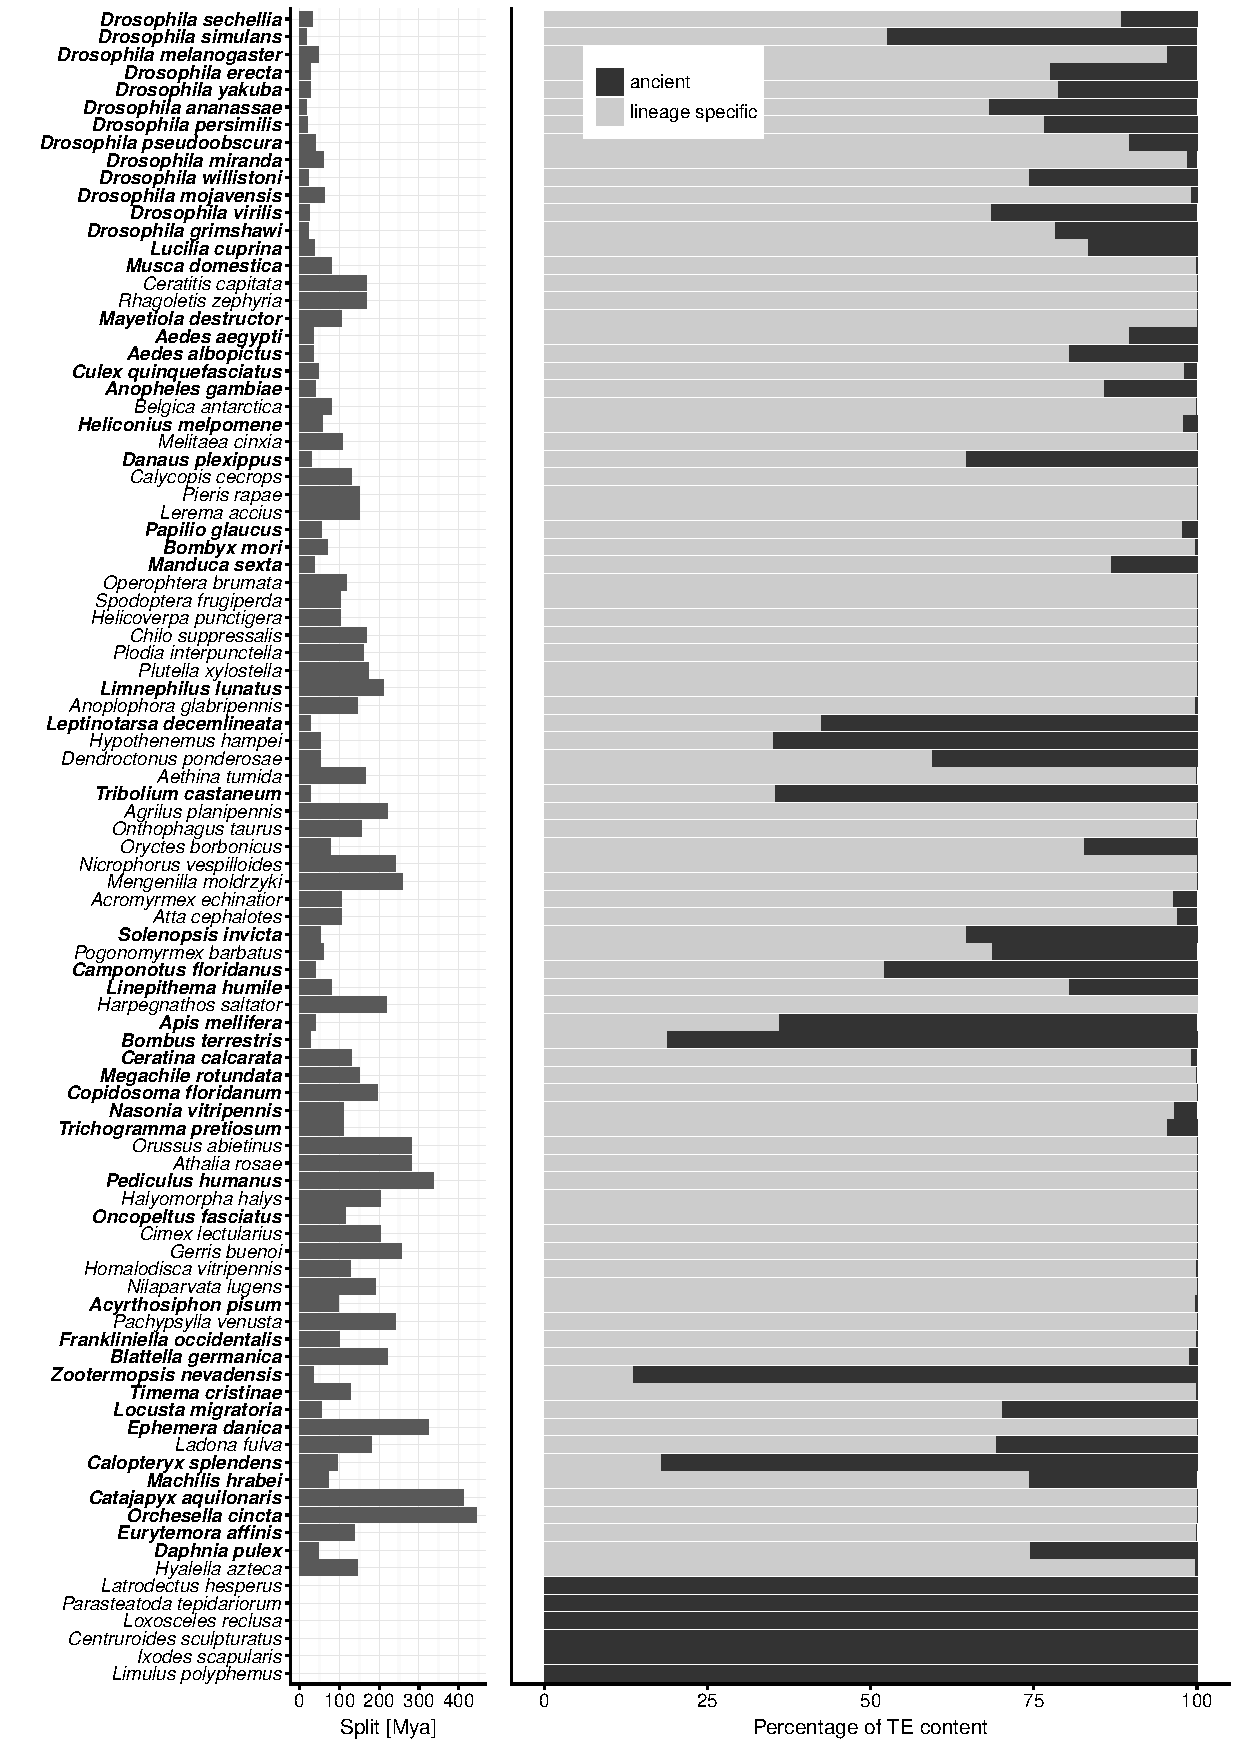
\includegraphics[width=\textwidth]{agesplit+ages}
\caption[Most insect TEs are clade-specific]{Most insect transposable elements are clade-specific when analyzed at order level. TE age was determined from the RepeatMasker \citep{Smit2015} annotation using the intra-TE-family Kimura distances and order-specific nucleotide substitution rates based on data from \citet{Misof2014}. TE copies were classified as ``ancient'' if they were older (more divergent) than the clade the host belongs to. Bold font face denotes species for which ancestral genome size inferences and branch length estimates are available.}
\label{fig:agesplit}
\end{figure}

\begin{figure}[h!]
\centering
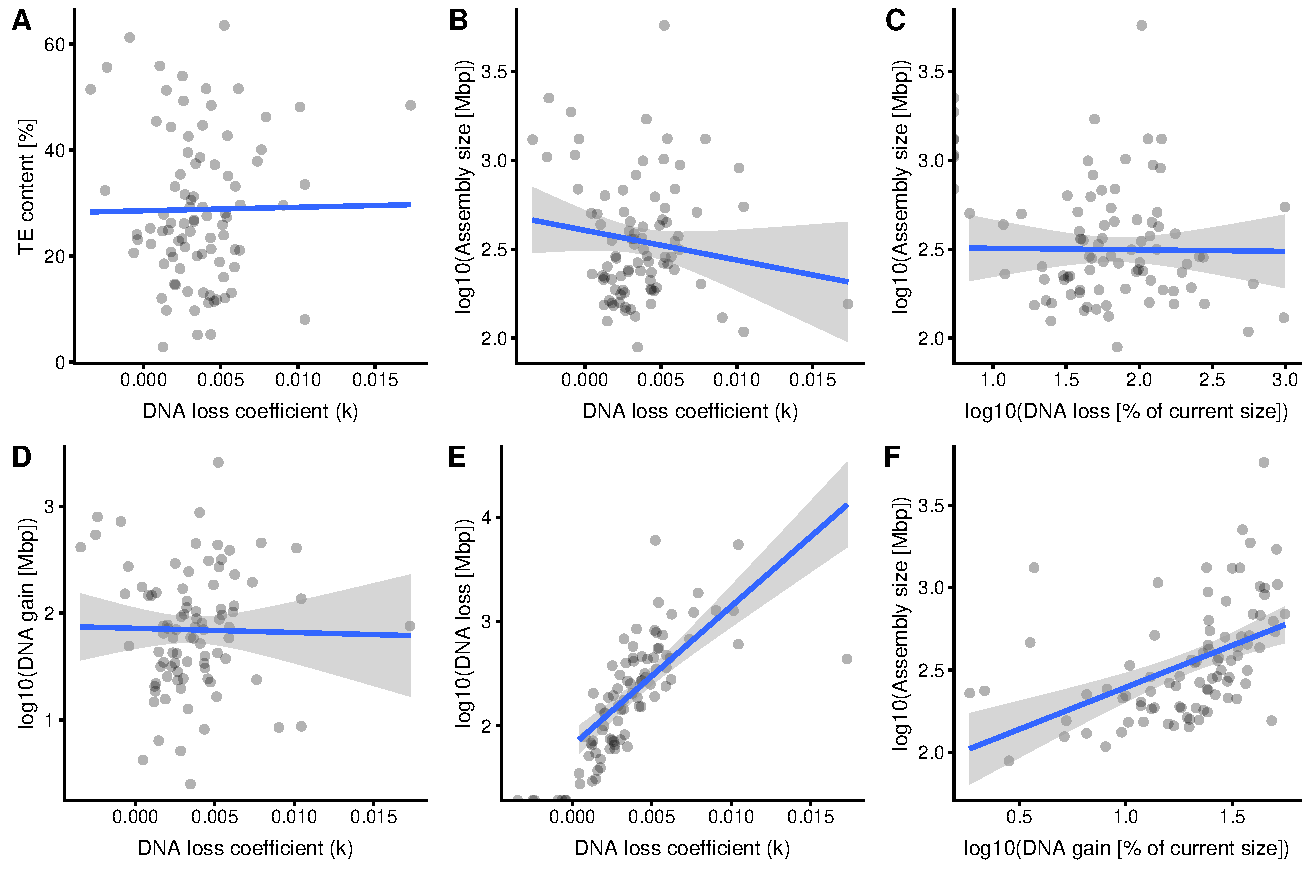
\includegraphics[width=\textwidth]{loss-coefficient-plots}
\rule{\textwidth}{0.2pt}

\bigskip

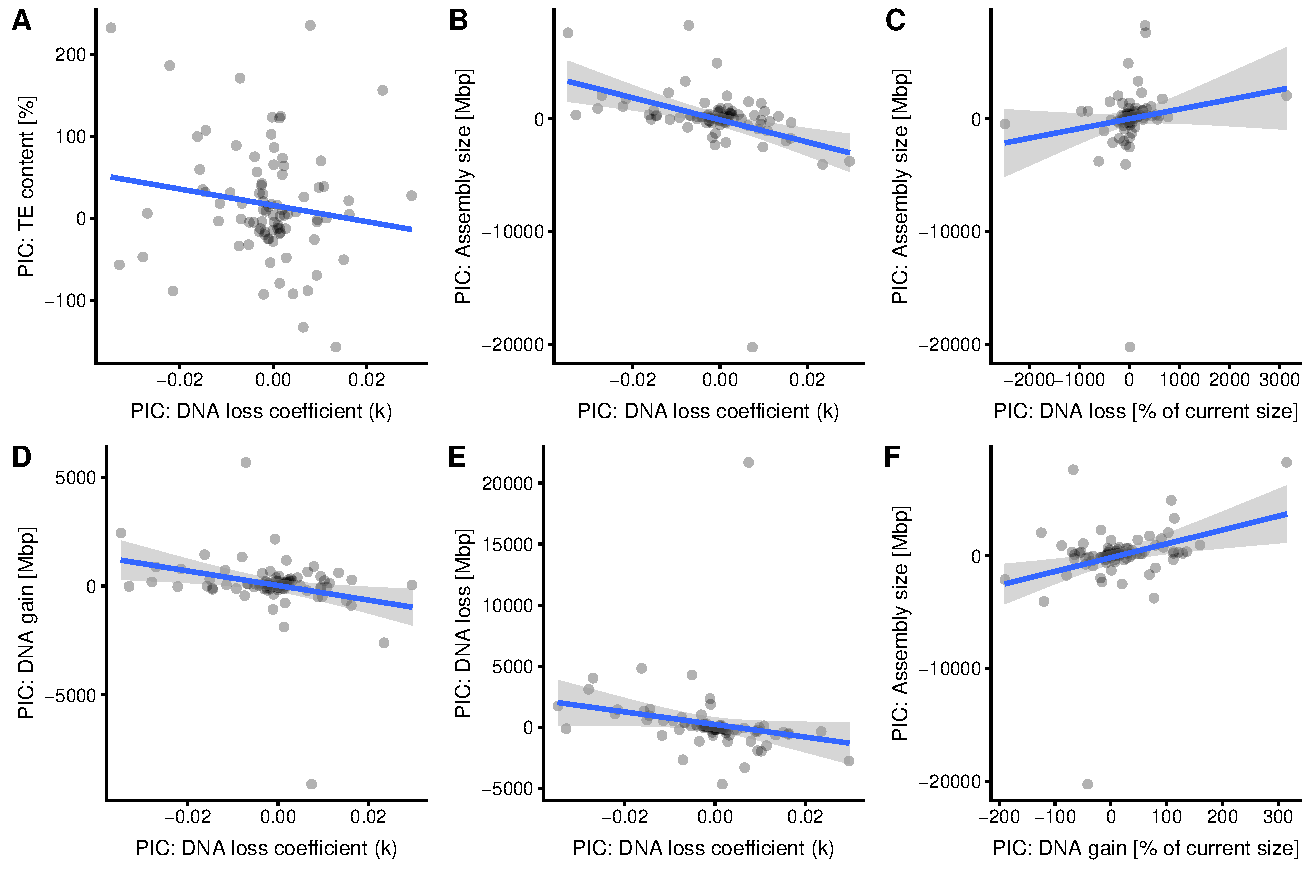
\includegraphics[width=\textwidth]{loss-coefficient-plots-PICs}
\caption[DNA loss coefficient correlations, with and without PIC]{Insect genome size dynamics and TE content are governed by the DNA loss coefficient. Top: without phylogenetic independent contrasts (PIC), bottom: with PIC. A: While TE content determines the genome size (Figure \ref{fig:te-content-vs-size}), the TE content is not dependent on the DNA loss coefficient $k$. There is no correlation despite a visible trend in the regression (Pearson, $p = 0.15$). Obviously, genome (assembly) size decreases with higher $k$ (B, $p = 0.0002$), as does the amount of DNA gained (D, $p = 0.01$). Surprisingly, the assembly size appears to remain more or less stable despite increasing amounts of DNA loss (C). A strong negative correlation is, however, found by testing for it (section \ref{sec:correlation-tests}; $p \ll 0.005$).}
\label{fig:loss-coefficient}
\end{figure}

\begin{figure}
\centering
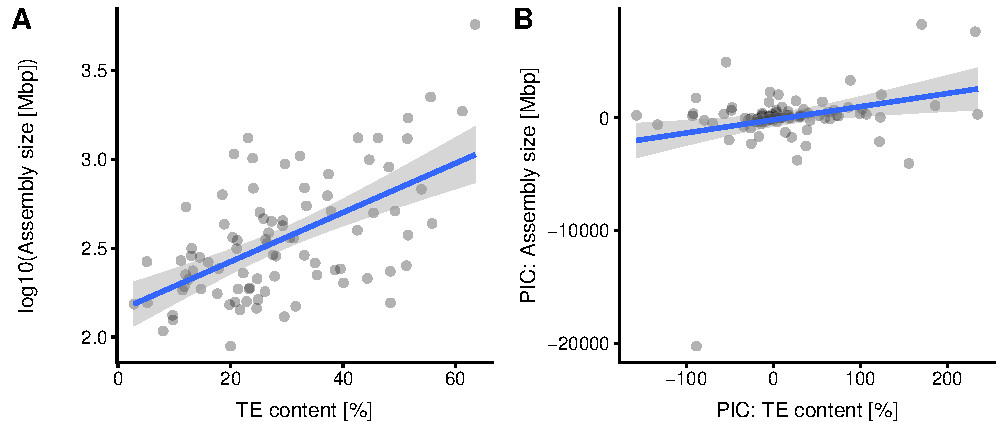
\includegraphics[width=\textwidth]{te-content-vs-size}
\caption[TE content is a predictor for genome size]{TE content is a predictor for genome size. Dots: individual measurements; blue line: linear regression; shaded area: confidence interval. PIC: phylogenetic independent contrast \citep{Felsenstein1985}}
\label{fig:te-content-vs-size}
\end{figure}

\begin{figure}[h!]
\centering
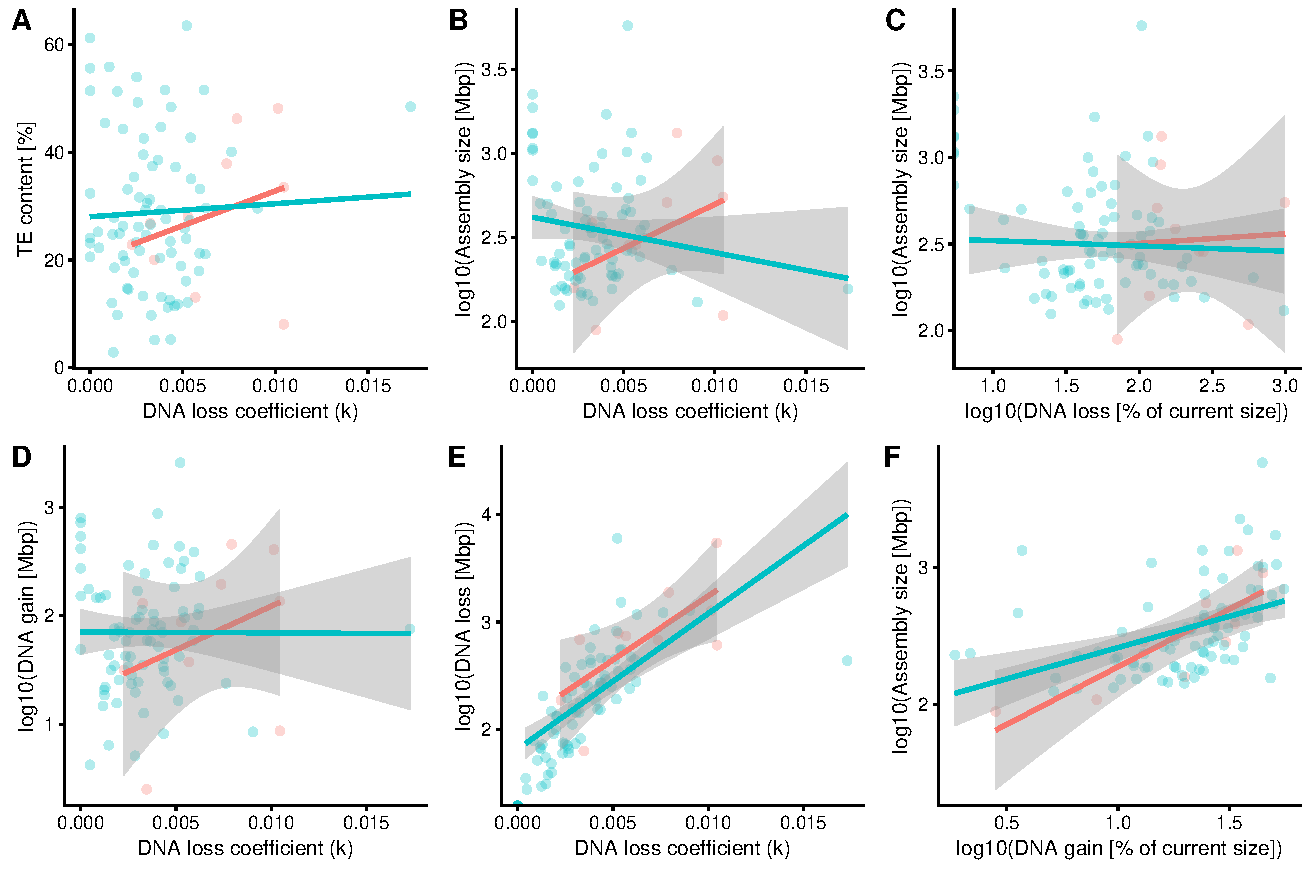
\includegraphics[width=\textwidth]{loss-coeffi-flightless}
\caption[TE content is a predictor for genome size, irrespective of flight ability]{The same as Fig. \ref{fig:te-content-vs-size}. Red: flightless; blue: flying}
\label{fig:loss-coefficient-plots-flight}
\end{figure}

\begin{figure}[h!]
\centering
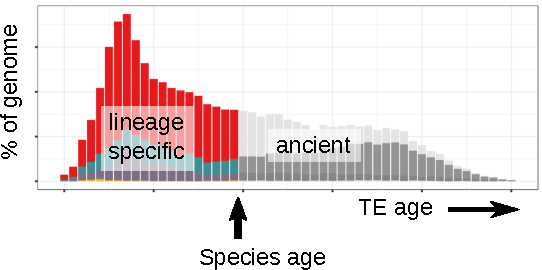
\includegraphics[width=\textwidth]{ancient-lineage-specific}
\caption[TE age classification explanation]{The age classification analysis splits the repeat landscape into the ancestral and the lineage-specific parts. The further to the right the species' age is, the greater the lineage-specific fraction of the TE content. If the species is older than the oldest TE copy on the landscape, it will have 0 \% ancestral TEs.}
\label{fig:ancient-lineage-specific}
\end{figure}

\clearpage

\section{Data sources}

\subsection{Genome assemblies}

\begin{center}
\tabcolsep=3pt
\begin{longtable}{lllp{12em}}
\caption[NCBI accession numbers and references for the genome assemblies]{NCBI accession numbers and references for the genome assemblies.} \label{tab:genome-assemblies} \\

\footnotesize
\endfirsthead

\multicolumn{2}{c}{%
{\tablename\ \thetable{} --continued}} \\
\toprule
Species & Order  & NCBI Accession & Reference \\
\midrule
\endhead

\bottomrule
\endfoot


\toprule
Species                              & Order           & NCBI Accession   & Reference \\
\midrule
\species{Drosophila yakuba}          & Diptera         & GCA\_000005975.1 & \citet{Drosophila12GenomesConsortium2007} \\
\species{Drosophila simulans}        & Diptera         & GCA\_000754195.2 & \citet{Drosophila12GenomesConsortium2007} \\
\species{Drosophila sechellia}       & Diptera         & GCF\_000005215.3 & \citet{Drosophila12GenomesConsortium2007} \\
\species{Drosophila melanogaster}    & Diptera         & GCA\_000001215.4 & \citet{Adams2000} \\
\species{Drosophila erecta}          & Diptera         & GCF\_000005135.1 & \citet{Drosophila12GenomesConsortium2007} \\
\species{Drosophila ananassae}       & Diptera         & GCF\_000005115.1 & \citet{Drosophila12GenomesConsortium2007} \\
\species{Drosophila pseudoobscura}   & Diptera         & GCF\_000001765.3 & \citet{Drosophila12GenomesConsortium2007} \\
\species{Drosophila persimilis}      & Diptera         & GCF\_000005195.2 & \citet{Drosophila12GenomesConsortium2007} \\
\species{Drosophila miranda}         & Diptera         & GCA\_000269505.2 & \citet{McGaugh2012} \\
\species{Drosophila willistoni}      & Diptera         & GCF\_000005925.1 & \citet{Drosophila12GenomesConsortium2007} \\
\species{Drosophila virilis}         & Diptera         & GCF\_000005245.1 & \citet{Drosophila12GenomesConsortium2007} \\
\species{Drosophila mojavensis}      & Diptera         & GCF\_000005175.2 & \citet{Drosophila12GenomesConsortium2007} \\
\species{Drosophila grimshawi}       & Diptera         & GCF\_000005155.2 & \citet{Drosophila12GenomesConsortium2007} \\
\species{Rhagoletis zephyria}        & Diptera         & GCA\_001687245.1 & \citet{Drosophila12GenomesConsortium2007} \\
\species{Ceratitis capitata}         & Diptera         & GCA\_000347755.2 & \citet{Papanicolaou2016} \\
\species{Lucilia cuprina}            & Diptera         & GCA\_000699065.1 & i5k Initiative \\
\species{Musca domestica}            & Diptera         & GCF\_000371365.1 & \citet{Scott2014} \\
\species{Culex quinquefasciatus}     & Diptera         & GCA\_000209185.1 & \citet{Arensburger2010} \\
\species{Aedes albopictus}           & Diptera         & GCA\_001444175.2 & \citet{Chen2015} \\
\species{Aedes aegypti}              & Diptera         & GCA\_000004015.1 & \citet{Nene2007} \\
\species{Anopheles gambiae}          & Diptera         & GCA\_000005575.1 & \citet{Holt2002} \\
\species{Belgica antarctica}         & Diptera         & GCA\_000775305.1 & \citet{Kelley2014} \\
\species{Mayetiola destructor}       & Diptera         & GCA\_000149185.1 & \citet{Zhao2015} \\
\species{Papilio glaucus}            & Lepidoptera     & GCA\_000931545.1 & \citet{Cong2015} \\
\species{Melitaea cinxia}            & Lepidoptera     & GCA\_000716385.1 & \citet{Ahola2014} \\
\species{Heliconius melpomene}       & Lepidoptera     & GCA\_000313835.2 & \citet{TheHeliconiusGenomeConsortium2012} \\
\species{Danaus plexippus}           & Lepidoptera     & GCA\_000235995.1 & \citet{Zhan2011} \\
\species{Calycopis cecrops}          & Lepidoptera     & GCA\_001625245.1 & \citet{Cong2016} \\
\species{Pieris rapae}               & Lepidoptera     & GCA\_001856805.1 & \citet{Shen2016} \\
\species{Lerema accius}              & Lepidoptera     & GCA\_001278395.1 & \citet{Cong2015a} \\
\species{Manduca sexta}              & Lepidoptera     & GCA\_000262585.1 & \citet{Kanost2016} \\
\species{Plutella xylostella}        & Lepidoptera     & GCA\_000325945.1 & \citet{You2013} \\
\species{Spodoptera frugiperda}      & Lepidoptera     & GCA\_000753635.2 & \citet{Gouin2017} \\
\species{Helicoverpa punctigera}     & Lepidoptera     &                  & i5k Initiative \\
\species{Chilo suppressalis}         & Lepidoptera     & GCA\_000636095.1 & \citet{Yin2014} \\
\species{Operophtera brumata}        & Lepidoptera     & GCA\_001266575.1 & \citet{Derks2015} \\
\species{Plodia interpunctella}      & Lepidoptera     & GCA\_900182495.1 & \citet{Paterson2017} \\
\species{Bombyx mori}                & Lepidoptera     & GCF\_000151625.1 & \citet{InternationalSilkwormGenomeConsortium2008} \\
\species{Limnephilus lunatus}        & Trichoptera     & GCA\_000648945.1 & i5k Initiative \\
\species{Aethina tumida}             & Coleoptera      & GCF\_001937115.1 & \citet{Evans2018} \\
\species{Anoplophora glabripennis}   & Coleoptera      & GCA\_000390285.1 & i5k Initiative \\
\species{Leptinotarsa decemlineata}  & Coleoptera      & GCA\_000500325.1 & i5k Initiative \\
\species{Tribolium castaneum}        & Coleoptera      & GCA\_000002335.2 & \citet{TriboliumGenomeSequencingConsortium2008} \\
\species{Agrilus planipennis}        & Coleoptera      & GCA\_000699045.1 & i5k Initiative \\
\species{Oryctes borbonicus}         & Coleoptera      & GCA\_001443705.1 & \citet{Meyer2016} \\
\species{Onthophagus taurus}         & Coleoptera      & GCA\_000648695.1 & i5k Initiative \\
\species{Dendroctonus ponderosae}    & Coleoptera      & GCF\_000355655.1 & \citet{Keeling2013} \\
\species{Hypothenemus hampei}        & Coleoptera      & GCA\_001012855.1 & \citet{Vega2015} \\
\species{Nicrophorus vespilloides}   & Coleoptera      & GCF\_001412225.1 & \citet{Cunningham2015} \\
\species{Mengenilla moldrzyki}       & Strepsiptera    & GCA\_000281935.1 & \citet{Niehuis2012} \\
\species{Pogonomyrmex barbatus}      & Hymenoptera     & GCA\_000187915.1 & \citet{Smith2011} \\
\species{Solenopsis invicta}         & Hymenoptera     & GCA\_000188075.1 & \citet{Wurm2011} \\
\species{Acromyrmex echinatior}      & Hymenoptera     & GCA\_000204515.1 & \citet{Nygaard2011} \\
\species{Atta cephalotes}            & Hymenoptera     & GCA\_000143395.2 & \citet{Suen2011} \\
\species{Harpegnathos saltator}      & Hymenoptera     & GCA\_000147195.1 & \citet{Bonasio2010} \\
\species{Camponotus floridanus}      & Hymenoptera     & GCA\_000147175.1 & \citet{Bonasio2010} \\
\species{Linepithema humile}         & Hymenoptera     & GCA\_000217595.1 & \citet{Smith2011a} \\
\species{Megachile rotundata}        & Hymenoptera     & GCF\_000220905.1 & \citet{Robinson2014} \\
\species{Ceratina calcarata}         & Hymenoptera     & GCF\_001652005.1 & \citet{Rehan2016} \\
\species{Bombus terrestris}          & Hymenoptera     & GCA\_000214255.1 & \citet{Sadd2015} \\
\species{Apis mellifera}             & Hymenoptera     & GCA\_000002195.1 & \citet{Honeybee2006} \\
\species{Nasonia vitripennis}        & Hymenoptera     & GCA\_000002325.2 & \citet{Werren2010} \\
\species{Copidosoma floridanum}      & Hymenoptera     & GCA\_000648655.1 & i5k Initiative \\
\species{Trichogramma pretiosum}     & Hymenoptera     & GCA\_000599845.2 & i5k Initiative \\
\species{Orussus abietinus}          & Hymenoptera     & GCA\_000612105.1 & i5k Initiative \\
\species{Athalia rosae}              & Hymenoptera     & GCA\_000344095.1 & i5k Initiative \\
\species{Pediculus humanus}          & Psocodea        & GCA\_000006295.1 & \citet{Kirkness2010} \\
\species{Halyomorpha halys}          & Heteroptera     & GCA\_000696795.1 & i5k Initiative \\
\species{Oncopeltus fasciatus}       & Heteroptera     & GCA\_000696205.1 & i5k Initiative \\
\species{Cimex lectularius}          & Heteroptera     & GCA\_000648675.1 & \citet{Rosenfeld2016} \\
\species{Gerris buenoi}              & Heteroptera     & GCA\_001010745.1 & i5k Initiative \\
\species{Nilaparvata lugens}         & Auchenorrhyncha & GCA\_000757685.1 & \citet{Xue2014} \\
\species{Homalodisca vitripennis}    & Auchenorrhyncha & GCA\_000696855.1 & i5k Initiative \\
\species{Pachypsylla venusta}        & Sternorrhyncha  & GCA\_000695645.1 & i5k Initiative \\
\species{Acyrthosiphon pisum}        & Sternorrhyncha  & GCA\_000142985.2 & \citet{TheInternationalAphidGenomicsConsortium2010} \\
\species{Frankliniella occidentalis} & Thysanoptera    & GCA\_000697945.1 & i5k Initiative \\
\species{Blattella germanica}        & Blattodea       & GCA\_000762945.1 & i5k Initiative \\
\species{Zootermopsis nevadensis}    & Isoptera        & GCA\_000696155.1 & \citet{Terrapon2014} \\
\species{Timema cristinae}           & Phasmatodea     & GCA\_002009905.3 & i5k Initiative \\
\species{Locusta migratoria}         & Orthoptera      & GCA\_000516895.1 & \citet{Wang2014} \\
\species{Ephemera danica}            & Ephemeroptera   & GCA\_000507165.1 & i5k Initiative \\
\species{Calopteryx splendens}       & Odonata         & GCA\_002093875.1 & i5k Initiative \\
\species{Ladona fulva}               & Odonata         & GCA\_000376725.1 & i5k Initiative \\
\species{Machilis hrabei}            & Archaeognatha   &                  & i5k Initiative \\
\species{Catajapyx aquilonaris}      & Diplura         & GCA\_000934665.1 & i5k Initiative \\
\species{Orchesella cincta}          & Collembola      & GCA\_001718145.1 & \citet{Faddeeva-Vakhrusheva2016} \\
\species{Hyalella azteca}            & Copepoda        &                  & i5k Initiative \\
\species{Eurytemora affinis}         & Branchiopoda    & GCA\_000591075.1 & \citet{Eyun2017} \\
\species{Daphnia pulex}              & Malacostraca    & GCA\_000187875.1 & \citet{Colbourne2011} \\
\species{Strigamia maritima}         & Myriapoda       & GCA\_000239455.1 & \citet{Chipman2014} \\
\species{Latrodectus hesperus}       & Araneae         & GCA\_000697925.1 & i5k Initiative \\
\species{Parasteatoda tepidariorum}  & Araneae         & GCA\_000365465.2 & \citet{Schwager2017} \\
\species{Loxosceles reclusa}         & Araneae         & GCA\_001188405.1 & i5k Initiative \\
\species{Centruroides sculpturatus}  & Scorpionidae    & GCA\_000671375.1 & \citet{Schwager2017} \\
\species{Ixodes scapularis}          & Ixodida         & GCA\_000208615.1 & \citet{Gulia-Nuss2016} \\
\species{Limulus polyphemus}         & Xiphosura       & GCA\_000517525.1 & \citet{Simpson2017} \\
\end{longtable}
\end{center}

\subsection{Insect genome size estimates}

We estimated genome sizes of eight additional species using either flow cytometry (FCM) or a \textit{k}-mer peak method adopted from \citep{Hozza2015}.
For \textit{k}-mer estimates, we downloaded genomic reads from i5k FTP server for \species{Limnephilus lunatus} and \species{Catajapyx aquilonaris}:

\begin{description}
	\item[\species{Catajapyx aquilonaris}:] \url{ftp://ftp.hgsc.bcm.edu/I5K-pilot/Silvestris_Northern_Forcepstail/genomic_sequence/Caqu_1Kb_1_sequence.txt.bz2}
	\item[\species{Limnephilus lunatus}:] \url{ftp://ftp.hgsc.bcm.edu/I5K-pilot/Caddisfly/genomic_sequence/Llun_8kb_1_sequence.txt.bz2}
\end{description}

For \species{Stylops ovinae}, we used our own (unpublished) genomic short reads.

Using flow cytometry, we estimated the genome size for an additional 9 species. The results are listed in table \ref{tab:genome-size-estimates} on page \pageref{tab:genome-size-estimates}.

\begin{table}[htb!]
\centering
\caption[Genome size estimates]{Genome size estimates. The \textit{c}-value (in picogram DNA per haploid cell) is converted to a value in Mbp by calculating $c \times 978$ \citep{Dolezel2003}. Note that \species{Stylops ater} is a synonym for \species{S. ovinae}. FCM: flow cytometry. }
\label{tab:genome-size-estimates}
\begin{tabular}{@{}lllrrl@{}}
\toprule
Order         & Family        & Species                         & c-value      & Mbp       & Method \\ \midrule
Diplura       & Japygidae     & \species{Catajapyx aquilonaris} & 0.316        & 308.855   & 25-mer \\
Thysanura     & Lepismatidae  & \species{Thermobia domestica}   & 3.982        & 3894.055  & FCM    \\
Thysanura     & Lepismatidae  & \species{Thermobia domestica}   & 3.837        & 3752.976  & FCM    \\
Thysanura     & Lepismatidae  & \species{Thermobia domestica}   & 2.000        & 1956.000  & FCM    \\
Ephemeroptera & Ephemeridae   & \species{Ephemera danica}       & 0.413        & 403.741   & FCM    \\
Ephemeroptera & Ephemeridae   & \species{Ephemera danica}       & 0.427        & 417.919   & FCM    \\
Ephemeroptera & Ephemeridae   & \species{Ephemera danica}       & 0.454        & 444.068   & FCM    \\
Ephemeroptera & Ephemeridae   & \species{Ephemera danica}       & 0.433        & 423.355   & FCM    \\
Ephemeroptera & Ephemeridae   & \species{Ephemera danica}       & 0.480        & 469.614   & FCM    \\
Ephemeroptera & Ephemeridae   & \species{Ephemera danica}       & 0.462        & 451.856   & FCM    \\
Ephemeroptera & Ephemeridae   & \species{Ephemera danica}       & 0.411        & 401.903   & FCM    \\
Ephemeroptera & Ephemeridae   & \species{Ephemera danica}       & 0.400        & 391.626   & FCM    \\
Mecoptera     & Panorpidae    & \species{Panorpa germanica}     & 0.591        & 578.002   & FCM    \\
Mecoptera     & Panorpidae    & \species{Panorpa germanica}     & 0.598        & 584.661   & FCM    \\
Megaloptera   & Sialidae      & \species{Sialis lutaria}        & 0.366        & 358.383   & FCM    \\
Megaloptera   & Sialidae      & \species{Sialis lutaria}        & 0.407        & 397.908   & FCM    \\
Megaloptera   & Sialidae      & \species{Sialis lutaria}        & 0.393        & 384.185   & FCM    \\
Megaloptera   & Sialidae      & \species{Sialis lutaria}        & 0.403        & 393.989   & FCM    \\
Neuroptera    & Chrysopidae   & \species{Chrysopa perla}        & 0.699        & 683.460   & FCM    \\
Neuroptera    & Chrysopidae   & \species{Chrysopa perla}        & 0.694        & 678.502   & FCM    \\
Neuroptera    & Chrysopidae   & \species{Chrysopa perla}        & 0.708        & 692.763   & FCM    \\
Neuroptera    & Chrysopidae   & \species{Chrysopa perla}        & 0.677        & 661.918   & FCM    \\
Neuroptera    & Chrysopidae   & \species{Chrysopa perla}        & 0.709        & 693.076   & FCM    \\
Neuroptera    & Chrysopidae   & \species{Chrysopa perla}        & 0.707        & 691.567   & FCM    \\
Strepsiptera  & Stylopidae    & \species{Stylops ater}          & 0.109        & 106.583   & FCM    \\
Strepsiptera  & Stylopidae    & \species{Stylops ovinae}        & 0.055        & 54.243    & 17-mer \\
Trichoptera   & Limnephilidae & \species{Limnephilus lunatus}   & 2.567        & 2510.874  & 17-mer \\ \bottomrule
\end{tabular}
\end{table}


\subsection{COI barcode sequences}

For the species that were part of our TE analysis, but were not represented in the BOLD database (Table \ref{tab:species-not-in-bold-but-in-tree} on page \pageref{tab:species-not-in-bold-but-in-tree}), we dowloaded COI sequences from NCBI Genbank by searching for ``species\_name COI''. In the cases where multiple sequences were returned, we selected the longest one. If there were multiple sequences with the longest length, we selected one at random.
For \species{Pachypsylla venusta}, the complete mitochondrial genome was available, but not just the COI sequence. We used the COI sequence of the closely related species \species{Bemisia tabaci} in an alignment using MAFFT and cropped the \species{P. venusta} sequence to the length of the \species{B. tabaci} COI sequence.

\begin{center}
\begin{longtable}{llll}
\caption{Species not represented in the BOLD database}
\label{tab:species-not-in-bold-but-in-tree}

\footnotesize
\endfirsthead

\multicolumn{2}{c}{%
{\tablename\ \thetable{} --continued}} \\
\toprule
Order & Family  & Genus & Species \\
\midrule
\endhead

\bottomrule
\endfoot


\toprule
Order & Family & Genus & Species \\
\midrule
Chelicerata & Buthidae & Centruroides & \species{C. sculpturatus} \\
Chelicerata & Ixodidae & Ixodes & \species{I. scapularis} \\
Chelicerata & Limulidae & Limulus & \species{L. polyphemus} \\
Chelicerata & Sicariidae & Loxosceles & \species{L. reclusa} \\
Chelicerata & Theridiidae & Latrodectus & \species{L. hesperus} \\
Chelicerata & Theridiidae & Parasteatoda & \species{P. tepidariorum} \\
Coleoptera & Buprestidae & Agrilus & \species{A. planipennis} \\
Coleoptera & Cerambycidae & Anoplophora & \species{A. glabripennis} \\
Coleoptera & Curculionidae & Dendroctonus & \species{D. ponderosae} \\
Coleoptera & Curculionidae & Hypothenemus & \species{H. hampei} \\
Coleoptera & Nitidulidae & Aethina & \species{A. tumida} \\
Coleoptera & Scarabaeidae & Onthophagus & \species{O. taurus} \\
Coleoptera & Scarabaeidae & Oryctes & \species{O. borbonicus} \\
Coleoptera & Silphidae & Nicrophorus & \species{N. vespilloides} \\
Crustacea & Dogielinotidae & Hyalella & \species{H. azteca} \\
Diptera & Chironomidae & Belgica & \species{B. antarctica} \\
Diptera & Tephritidae & Ceratitis & \species{C. capitata} \\
Diptera & Tephritidae & Rhagoletis & \species{R. zephyria} \\
Hemiptera & Aphalaridae & Pachypsylla & \species{P. venusta} \\
Hemiptera & Cicadellidae & Homalodisca & \species{H. vitripennis} \\
Hemiptera & Cimicidae & Cimex & \species{C. lectularius} \\
Hemiptera & Delphacidae & Nilaparvata & \species{N. lugens} \\
Hemiptera & Gerridae & Gerris & \species{G. buenoi} \\
Hemiptera & Miridae & Halyomorpha & \species{H. halys} \\
Hymenoptera & Formicidae & Acromyrmex & \species{A. echinatior} \\
Hymenoptera & Formicidae & Atta & \species{A. cephalotes} \\
Hymenoptera & Formicidae & Harpegnathos & \species{H. saltator} \\
Hymenoptera & Formicidae & Pogonomyrmex & \species{P. barbatus} \\
Hymenoptera & Orussidae & Orussus & \species{O. abietinus} \\
Hymenoptera & Tenthredinidae & Athalia & \species{A. rosae} \\
Lepidoptera & Crambidae & Chilo & \species{C. suppressalis} \\
Lepidoptera & Geometridae & Operophtera & \species{O. brumata} \\
Lepidoptera & Hesperidae & Lerema & \species{L. accius} \\
Lepidoptera & Lycaenidae & Calycopis & \species{C. cecrops} \\
Lepidoptera & Noctuidae & Helicoverpa & \species{H. punctigera} \\
Lepidoptera & Noctuidae & Spodoptera & \species{S. frugiperda} \\
Lepidoptera & Nymphalidae & Melitaea & \species{M. cinxia} \\
Lepidoptera & Pieridae & Pieris & \species{P. rapae} \\
Lepidoptera & Plutellidae & Plutella & \species{P. xylostella} \\
Lepidoptera & Pyralidae & Plodia & \species{P. interpunctella} \\
Myriapoda & Linotaeniidae & Strigamia & \species{S. maritima} \\
Odonata & Libellulidae & Ladona & \species{L. fulva} \\
Strepsiptera & Mengenillidae & Mengenilla & \species{M. moldrzyki} \\
\end{longtable}
\end{center}


\begin{longtable}{lrr}
\caption[Divergence times and MRCA splits]{Divergence times in Mya and MRCA split node numbers in the ancestral reconstruction phylogeny.}\label{tab:species-divergence-times} \\

\footnotesize
\endfirsthead

\multicolumn{2}{c}{%
{\tablename\ \thetable{} --continued}} \\
\toprule
Species & MRCA node  & Age [Mya] \\
\midrule
\endhead

\bottomrule
\endfoot

\toprule
Species                              & MRCA node & Age                \\ \midrule
\species{Drosophila yakuba}          & 765       & 21.44269125067723  \\
\species{Drosophila simulans}        & 763       & 12.865614687731181 \\
\species{Drosophila sechellia}       & 762       & 25.731229532150792 \\
\species{Drosophila melanogaster}    & 761       & 38.59684437657046  \\
\species{Drosophila erecta}          & 766       & 21.44269125067723  \\
\species{Drosophila ananassae}       & 786       & 12.603051120340638 \\
\species{Drosophila pseudoobscura}   & 774       & 31.507628033726974 \\
\species{Drosophila persimilis}      & 775       & 15.75381393851842  \\
\species{Drosophila miranda}         & 773       & 47.26144212893445  \\
\species{Drosophila willistoni}      & 793       & 16.804068211792014 \\
\species{Drosophila virilis}         & 799       & 20.164881885285638 \\
\species{Drosophila mojavensis}      & 803       & 49.99210323877088  \\
\species{Drosophila grimshawi}       & 812       & 18.904576757561074 \\
\species{Rhagoletis zephyria}        & 844       & 118.0306991714125  \\
\species{Ceratitis capitata}         & 844       & 118.0306991714125  \\
\species{Lucilia cuprina}            & 839       & 25.797218874700604 \\
\species{Musca domestica}            & 841       & 55.27975490960449  \\
\species{Culex quinquefasciatus}     & 887       & 25.92919755978727  \\
\species{Aedes albopictus}           & 882       & 18.52085535580352  \\
\species{Aedes aegypti}              & 882       & 18.52085535580352  \\
\species{Anopheles gambiae}          & 890       & 22.225026457795423 \\
\species{Belgica antarctica}         & 896       & 44.45005306974764  \\
\species{Mayetiola destructor}       & 868       & 66.61851738853375  \\
\species{Papilio glaucus}            & 963       & 36.555952942833926 \\
\species{Melitaea cinxia}            & 957       & 73.1119060406304   \\
\species{Heliconius melpomene}       & 959       & 36.555952942833926 \\
\species{Danaus plexippus}           & 960       & 18.277976393935717 \\
\species{Calycopis cecrops}          & 956       & 91.3898825895289   \\
\species{Pieris rapae}               & 955       & 109.66785913842705 \\
\species{Lerema accius}              & 955       & 109.66785913842705 \\
\species{Manduca sexta}              & 948       & 22.847470531160297 \\
\species{Plutella xylostella}        & 907       & 138.6079886790834  \\
\species{Spodoptera frugiperda}      & 914       & 63.97291776618124  \\
\species{Helicoverpa punctigera}     & 914       & 63.97291776618124  \\
\species{Chilo suppressalis}         & 908       & 127.9458356873252  \\
\species{Operophtera brumata}        & 913       & 74.63507075303869  \\
\species{Plodia interpunctella}      & 909       & 117.28368270046786 \\
\species{Bombyx mori}                & 954       & 45.69494121728309  \\
\species{Limnephilus lunatus}        & 906       & 175.29599553826313 \\
\species{Aethina tumida}             & 973       & 150.78055424458506 \\
\species{Anoplophora glabripennis}   & 975       & 130.67648032433073 \\
\species{Leptinotarsa decemlineata}  & 989       & 25.13009224299492  \\
\species{Tribolium castaneum}        & 1001      & 24.412089602985986 \\
\species{Agrilus planipennis}        & 968       & 201.04073904522096 \\
\species{Oryctes borbonicus}         & 1028      & 70.36425856356772  \\
\species{Onthophagus taurus}         & 1026      & 140.728517284458   \\
\species{Dendroctonus ponderosae}    & 995       & 46.90950565660398  \\
\species{Hypothenemus hampei}        & 995       & 46.90950565660398  \\
\species{Nicrophorus vespilloides}   & 966       & 221.14481296547535 \\
\species{Mengenilla moldrzyki}       & 964       & 241.24888688572963 \\
\species{Pogonomyrmex barbatus}      & 1054      & 57.31899918445174  \\
\species{Solenopsis invicta}         & 1056      & 50.95022147977727  \\
\species{Acromyrmex echinatior}      & 1055      & 101.90044311717185 \\
\species{Atta cephalotes}            & 1055      & 101.90044311717185 \\
\species{Harpegnathos saltator}      & 1039      & 210.1696640966345  \\
\species{Camponotus floridanus}      & 1048      & 38.21266607042867  \\
\species{Linepithema humile}         & 1060      & 76.42533229847476  \\
\species{Megachile rotundata}        & 1071      & 145.90290725855766 \\
\species{Ceratina calcarata}         & 1072      & 125.05963477053274 \\
\species{Bombus terrestris}          & 1082      & 26.054090452413732 \\
\species{Apis mellifera}             & 1084      & 39.08113575743005  \\
\species{Nasonia vitripennis}        & 1106      & 106.99546528091116 \\
\species{Copidosoma floridanum}      & 1103      & 187.24206435980705 \\
\species{Trichogramma pretiosum}     & 1113      & 106.99546528091116 \\
\species{Orussus abietinus}          & 1036      & 267.48866344165566 \\
\species{Athalia rosae}              & 1036      & 267.48866344165566 \\
\species{Pediculus humanus}          & 713       & 369.2516881752408  \\
\species{Halyomorpha halys}          & 1141      & 201.57612771302968 \\
\species{Oncopeltus fasciatus}       & 1151      & 113.38657176954973 \\
\species{Cimex lectularius}          & 1141      & 201.57612771302968 \\
\species{Gerris buenoi}              & 1139      & 251.97015968073242 \\
\species{Nilaparvata lugens}         & 1152      & 188.97761972110402 \\
\species{Homalodisca vitripennis}    & 1153      & 125.98507976147562 \\
\species{Pachypsylla venusta}        & 1122      & 237.57186483281725 \\
\species{Acyrthosiphon pisum}        & 1129      & 98.98827692163468  \\
\species{Frankliniella occidentalis} & 1156      & 98.98827692163474  \\
\species{Blattella germanica}        & 1178      & 272.80341460998403 \\
\species{Zootermopsis nevadensis}    & 1186      & 45.46723563615387  \\
\species{Timema cristinae}           & 1188      & 159.13532512306904 \\
\species{Locusta migratoria}         & 1173      & 68.20085353353676  \\
\species{Ephemera danica}            & 1189      & 396.1678512831885  \\
\species{Calopteryx splendens}       & 1220      & 121.05128778189425 \\
\species{Ladona fulva}               & 1194      & 231.09791318241201 \\
\species{Machilis hrabei}            & 1225      & 93.82705441726876  \\
\species{Catajapyx aquilonaris}      & 707       & 489.1119896305598  \\
\species{Orchesella cincta}          & 706       & 509.0887065396401  \\
\species{Hyalella azteca}            & 690       & 198.39953369400536 \\
\species{Eurytemora affinis}         & 632       & 183.13803108993875 \\
\species{Daphnia pulex}              & 640       & 63.95296313437109  \\
\species{Strigamia maritima}         &           & NA                 \\
\species{Latrodectus hesperus}       &           & NA                 \\
\species{Parasteatoda tepidariorum}  &           & NA                 \\
\species{Loxosceles reclusa}         &           & NA                 \\
\species{Centruroides sculpturatus}  &           & NA                 \\
\species{Ixodes scapularis}          &           & NA                 \\
\species{Limulus polyphemus}         &           & NA                 \\ \bottomrule
\end{longtable}


\section{TE age determination}

\subsection{Divergence times and substitution rates}

To obtain order-specific substitution rates, we calculated the weighted arithmetic mean as

\begin{equation}
	\bar{x}_w = \frac{\sum_{i=1}^{n}w_{i}x_{i}}{\sum_{i=1}^{n}w_i}
	\label{eqn:weighted-arithmetic-mean}
\end{equation}

with $n$ = number of branches in  the tree,
$w_i$ = branch substitution rate,
$t_i$ = branch time,
$x_i$ = $\frac{w_i}{t_i}$.

Thus, longer branches have a higher influence on the mean substitution rate than shorter branches. The results are listed in Table \ref{tab:order-divergence-times} (page \pageref{tab:order-divergence-times}). Note that for the TE age classification (``agesplit''), we used species-specific divergence times derived from the time-calibrated phylogeny, listed in Table \ref{tab:species-divergence-times}.

\subsection{DNA gain and loss}

Insect order divergence times were taken from \citet{Misof2014} and are listed in Table \ref{tab:order-divergence-times} (page \pageref{tab:order-divergence-times}). We used the upper and lower confidence interval as maximum and minimum age, respectively, for the time calibration of the ancestral genome size reconstruction tree. We used the splits listed in Table \ref{tab:calibration-points} (page \pageref{tab:calibration-points}) as calibration points to convert the ultrametric phylogeny into a chronogram.

The inferred amounts of DNA gain and loss are listed in Table \ref{tab:gain-loss} (page \pageref{tab:gain-loss}).

\subsubsection{Correlation tests under phylogenetic independent contrasts (PIC)}\label{sec:correlation-tests}


Some correlations are only apparent when correcting for phylogeny. This also shows the importance of considering the phylogeny when drawing conclusions in comparative studies. 

\clearpage

\paragraph{TE content and $k$:}

\begin{verbatim}
	Pearson's product-moment correlation

data:  pic.tes and pic.k
t = -1.9038, df = 85, p-value = 0.06032
alternative hypothesis: true correlation is not equal to 0
95 percent confidence interval:
 -0.396008539  0.008792809
sample estimates:
     cor 
-0.20223 
\end{verbatim}

\clearpage

\paragraph{Genome size and $k$:}

\begin{verbatim}
	Pearson's product-moment correlation

data:  pic.size and pic.k
t = -4.0119, df = 85, p-value = 0.0001291
alternative hypothesis: true correlation is not equal to 0
95 percent confidence interval:
 -0.5623912 -0.2056495
sample estimates:
       cor 
-0.3990127 
\end{verbatim}

\clearpage

\paragraph{DNA gain and $k$:}

\begin{verbatim}
	Pearson's product-moment correlation

data:  pic.gain and pic.k
t = -2.7991, df = 85, p-value = 0.006341
alternative hypothesis: true correlation is not equal to 0
95 percent confidence interval:
 -0.47225571 -0.08506429
sample estimates:
       cor 
-0.2905071 
\end{verbatim}

\clearpage

\paragraph{DNA loss and $k$:}

\begin{verbatim}
	Pearson's product-moment correlation

data:  pic.loss and pic.k
t = -2.1293, df = 85, p-value = 0.03612
alternative hypothesis: true correlation is not equal to 0
95 percent confidence interval:
 -0.41596621 -0.01510393
sample estimates:
       cor 
-0.2250362 
\end{verbatim}

\clearpage

\paragraph{DNA gain and genome (assembly) size:}

\begin{verbatim}
	Pearson's product-moment correlation

data:  pic.gain and pic.size
t = 24.438, df = 85, p-value < 2.2e-16
alternative hypothesis: true correlation is not equal to 0
95 percent confidence interval:
 0.9029451 0.9575565
sample estimates:
      cor 
0.9356325 
\end{verbatim}

\clearpage

\paragraph{DNA loss and genome (assembly) size:}

\begin{verbatim}
	Pearson's product-moment correlation

data:  pic.loss and pic.size
t = -9.1316, df = 85, p-value = 2.923e-14
alternative hypothesis: true correlation is not equal to 0
95 percent confidence interval:
 -0.7963161 -0.5788707
sample estimates:
       cor 
-0.7037099 
\end{verbatim}

\begin{center}
\begin{longtable}[t]{lrrrr}
\caption[DNA gain and loss]{The calculated DNA losses and gains in the 96 studied species show large
variation. DNA gain is defined as the amount of clade-specific TEs, while DNA loss is
calculated as the difference between ancestral clade genome size and ancestral DNA of
the species (assembly size – clade-specific TEs). Clade relationships after \citet{Misof2014},
intra-ordinal relationships based on published phylogenies listed in Table \ref{tab:phylogeny-sources}.}
\label{tab:gain-loss}

\footnotesize
\endfirsthead

\multicolumn{2}{c}{%
{\tablename\ \thetable{} --continued}} \\
\toprule
Species                    & Ancestral size {[}Mbp{]} & Assembly {[}Mbp{]} & Gain {[}Mbp{]} & loss {[}Mbp{]} \\
\midrule
\endhead

\bottomrule
\endfoot

\toprule
Species                    & Ancestral size {[}Mbp{]} & Assembly {[}Mbp{]} & Gain {[}Mbp{]} & loss {[}Mbp{]} \\ \midrule
\species{Drosophila yakuba}          & 253.38                   & 162.60             & 40.08          & 130.86         \\
\species{Drosophila simulans}        & 253.38                   & 124.61             & 12.16          & 140.94         \\
\species{Drosophila sechellia}       & 253.38                   & 157.25             & 39.16          & 135.29         \\
\species{Drosophila melanogaster}    & 253.38                   & 142.57             & 29.66          & 140.47         \\
\species{Drosophila erecta}          & 253.38                   & 145.08             & 31.48          & 139.77         \\
\species{Drosophila ananassae}       & 253.38                   & 213.92             & 94.87          & 134.33         \\
\species{Drosophila pseudoobscura}   & 253.38                   & 149.03             & 26.28          & 130.63         \\
\species{Drosophila persimilis}      & 253.38                   & 175.58             & 55.51          & 133.31         \\
\species{Drosophila miranda}         & 253.38                   & 132.59             & 12.85          & 133.65         \\
\species{Drosophila willistoni}      & 253.38                   & 223.61             & 79.19          & 108.96         \\
\species{Drosophila virilis}         & 253.38                   & 189.21             & 49.44          & 113.62         \\
\species{Drosophila mojavensis}      & 253.38                   & 180.21             & 42.21          & 115.39         \\
\species{Drosophila grimshawi}       & 253.38                   & 186.09             & 43.33          & 110.62         \\
\species{Rhagoletis zephyria}        & 346.78                   & 1045.32            & 122.69         & -575.85        \\
\species{Ceratitis capitata}         & 346.78                   & 440.70             & 386.49         & 292.57         \\
\species{Lucilia cuprina}            & 585.89                   & 379.07             & 539.20         & 746.02         \\
\species{Musca domestica}            & 585.89                   & 691.74             & 146.18         & 40.32          \\
\species{Culex quinquefasciatus}     & 606.87                   & 539.96             & 276.99         & 343.90         \\
\species{Aedes albopictus}           & 1011.02                  & 1776.29            & 987.68         & 222.41         \\
\species{Aedes aegypti}              & 1011.02                  & 1310.09            & 802.33         & 503.27         \\
\species{Anopheles gambiae}          & 1011.02                  & 252.44             & 50.54          & 809.12         \\
\species{Belgica antarctica}         & 149.71                   & 88.99              & 2.51           & 63.23          \\
\species{Mayetiola destructor}       & 156.92                   & 153.14             & 18.54          & 22.32          \\
\species{Papilio glaucus}            & 401.06                   & 361.20             & 99.63          & 139.49         \\
\species{Melitaea cinxia}            & 378.11                   & 361.02             & 112.72         & 129.81         \\
\species{Heliconius melpomene}       & 352.65                   & 269.65             & 82.52          & 165.51         \\
\species{Danaus plexippus}           & 330.92                   & 272.28             & 30.46          & 89.10          \\
\species{Calycopis cecrops}          & 363.37                   & 689.13             & 272.59         & -53.17         \\
\species{Pieris rapae}               & 368.94                   & 242.73             & 58.41          & 184.63         \\
\species{Lerema accius}              & 368.94                   & 289.62             & 51.91          & 131.23         \\
\species{Manduca sexta}              & 456.58                   & 399.66             & 106.07         & 162.99         \\
\species{Plutella xylostella}        & 472.47                   & 186.03             & 35.13          & 321.57         \\
\species{Spodoptera frugiperda}      & 687.01                   & 330.62             & 70.14          & 426.53         \\
\species{Helicoverpa punctigera}     & 687.01                   & 350.24             & 73.87          & 410.64         \\
\species{Chilo suppressalis}         & 471.68                   & 314.17             & 117.03         & 274.54         \\
\species{Operophtera brumata}        & 685.17                   & 624.73             & 307.85         & 368.29         \\
\species{Plodia interpunctella}      & 513.30                   & 364.62             & 74.27          & 222.95         \\
\species{Bombyx mori}                & 499.30                   & 431.73             & 183.81         & 251.39         \\
\species{Limnephilus lunatus}        & 544.65                   & 804.08             & 413.69         & 154.26         \\
\species{Aethina tumida}             & 657.89                   & 234.34             & 30.69          & 454.24         \\
\species{Anoplophora glabripennis}   & 710.89                   & 602.43             & 291.74         & 400.21         \\
\species{Leptinotarsa decemlineata}  & 688.55                   & 678.27             & 366.13         & 376.41         \\
\species{Tribolium castaneum}        & 234.88                   & 151.32             & 44.27          & 127.84         \\
\species{Agrilus planipennis}        & 627.58                   & 252.63             & 88.62          & 463.57         \\
\species{Oryctes borbonicus}         & 909.82                   & 423.77             & 125.37         & 611.42         \\
\species{Onthophagus taurus}         & 723.50                   & 238.61             & 95.65          & 580.53         \\
\species{Dendroctonus ponderosae}    & 1349.29                  & 201.82             & 40.01          & 1187.48        \\
\species{Hypothenemus hampei}        & 1349.29                  & 130.55             & 24.22          & 1242.96        \\
\species{Nicrophorus vespilloides}   & 581.20                   & 192.10             & 22.62          & 411.71         \\
\species{Mengenilla moldrzyki}       & 438.32                   & 155.73             & 75.48          & 358.07         \\
\species{Pogonomyrmex barbatus}      & 268.29                   & 220.21             & 32.03          & 80.11          \\
\species{Solenopsis invicta}         & 426.50                   & 354.73             & 117.46         & 189.23         \\
\species{Acromyrmex echinatior}      & 343.31                   & 288.58             & 80.40          & 135.13         \\
\species{Atta cephalotes}            & 343.31                   & 281.25             & 73.86          & 135.92         \\
\species{Harpegnathos saltator}      & 368.28                   & 283.10             & 70.01          & 155.19         \\
\species{Camponotus floridanus}      & 321.96                   & 224.63             & 28.21          & 125.53         \\
\species{Linepithema humile}         & 257.70                   & 213.27             & 25.64          & 70.07          \\
\species{Megachile rotundata}        & 476.16                   & 265.92             & 59.22          & 269.46         \\
\species{Ceratina calcarata}         & 476.16                   & 183.85             & 24.48          & 316.78         \\
\species{Bombus terrestris}          & 398.11                   & 236.41             & 27.08          & 188.77         \\
\species{Apis mellifera}             & 251.45                   & 229.11             & 11.74          & 34.09          \\
\species{Nasonia vitripennis}        & 426.41                   & 238.62             & 60.20          & 247.99         \\
\species{Copidosoma floridanum}      & 334.55                   & 454.98             & 175.59         & 55.16          \\
\species{Trichogramma pretiosum}     & 254.06                   & 181.15             & 26.68          & 99.59          \\
\species{Orussus abietinus}          & 358.53                   & 186.48             & 39.80          & 211.85         \\
\species{Athalia rosae}              & 358.53                   & 156.83             & 8.17           & 209.87         \\
\species{Pediculus humanus}          & 387.75                   & 108.40             & 8.70           & 288.06         \\
\species{Halyomorpha halys}          & 953.82                   & 1000.80            & 447.22         & 400.24         \\
\species{Oncopeltus fasciatus}       & 1833.80                  & 773.64             & 229.56         & 1289.72        \\
\species{Cimex lectularius}          & 953.82                   & 513.62             & 194.56         & 634.76         \\
\species{Gerris buenoi}              & 913.26                   & 653.32             & 244.59         & 504.52         \\
\species{Nilaparvata lugens}         & 1321.64                  & 1017.42            & 434.43         & 738.65         \\
\species{Homalodisca vitripennis}    & 2444.86                  & 1325.90            & 317.52         & 1436.48        \\
\species{Pachypsylla venusta}        & 605.50                   & 371.84             & 168.94         & 402.59         \\
\species{Acyrthosiphon pisum}        & 437.89                   & 499.89             & 146.41         & 84.40          \\
\species{Frankliniella occidentalis} & 411.61                   & 263.81             & 42.29          & 190.10         \\
\species{Blattella germanica}        & 1833.68                  & 1710.49            & 842.24         & 965.43         \\
\species{Zootermopsis nevadensis}    & 901.50                   & 464.44             & 43.52          & 480.58         \\
\species{Timema cristinae}           & 1850.01                  & 844.26             & 405.77         & 1411.51        \\
\species{Locusta migratoria}         & 9201.19                  & 5759.80            & 3658.54        & 7099.94        \\
\species{Ephemera danica}            & 1070.02                  & 399.55             & 109.20         & 779.68         \\
\species{Calopteryx splendens}       & 1174.90                  & 1324.05            & 226.06         & 76.92          \\
\species{Ladona fulva}               & 809.51                   & 948.04             & 191.87         & 53.34          \\
\species{Machilis hrabei}            & 2780.23                  & 1322.99            & 605.88         & 2063.13        \\
\species{Catajapyx aquilonaris}      & 1256.19                  & 311.13             & 87.38          & 1032.44        \\
\species{Orchesella cincta}          & 1273.33                  & 286.75             & 37.42          & 1024.00        \\
\species{Hyalella azteca}            & 5897.57                  & 596.63             & 136.37         & 5437.31        \\
\species{Eurytemora affinis}         & 906.42                   & 387.57             & 129.86         & 648.70         \\
\species{Daphnia pulex}              & 313.54                   & 158.61             & 42.48          & 197.41         \\
\species{Strigamia maritima}         & 2171.16                  & 173.60             & 73.69          & 2071.25        \\
\species{Latrodectus hesperus}       & 2171.16                  & 726.41             & 192.24         & 1636.99        \\
\species{Parasteatoda tepidariorum}  & 2171.16                  & 1141.93            & 442.18         & 1471.40        \\
\species{Loxosceles reclusa}         & 2171.16                  & 1793.28            & 1077.48        & 1455.35        \\
\species{Centruroides sculpturatus}  & 2171.16                  & 627.51             & 221.45         & 1765.10        \\
\species{Ixodes scapularis}          & 2171.16                  & 1388.47            & 707.90         & 1490.59        \\
\species{Limulus polyphemus}         & 2171.16                  & 1706.69            & 608.32         & 1072.79        \\
\end{longtable}
\end{center}

\begin{table}
\centering
\caption[Divergence times and clade-specific substitution rates]{Divergence times and clade-specific substitution rates for the arthropod orders in this study. Substitution rates are in substitutions $\times$ position$^{-1}$ $\times$ My$^{-1}$.}
\label{tab:order-divergence-times}
\begin{tabular}{@{}lllll@{}}
\toprule
Clade                      & Species & Divergence time [Mya] & Substitution rate \\ \midrule
Diptera                    & 23      & 157.83                    & 0.0067943                     \\
Lepidoptera                & 15      & 141.47                    & 0.0066874                     \\
Trichoptera                & 1       & 154.32                    & 0.004798                      \\
Coleoptera                 & 10      & 269.98                    & 0.0034029                     \\
Strepsiptera               & 1       & 107.56                    & 0.0069976                     \\
Hymenoptera                & 16      & 239.53                    & 0.0036226                     \\
Phthiraptera               & 1       & 187.33                    & 0.0059665                     \\
Hemiptera: Heteroptera     & 4       & 155.56                    & 0.0059329                     \\
Hemiptera: Auchenorrhyncha & 2       & 169.58                    & 0.0040139                     \\
Hemiptera: Sternorrhyncha  & 2       & 245.03                    & 0.0049467                     \\
Thysanoptera               & 1       & 119.93                    & 0.005508                      \\
Blattodea + Isoptera       & 1       & 172.98                    & 0.0019926                     \\
Isoptera                   & 1       & 135.83                    & 0.0011611                     \\
Phasmatodea                & 1       & 124.71                    & 0.0039888                     \\
Orthoptera                 & 1       & 202.7                     & 0.0037212                     \\
Ephemeroptera              & 1       & 178.82                    & 0.00412                       \\
Odonata                    & 2       & 234.73                    & 0.0013438                     \\
Archaeognatha              & 1       & 145.65                    & 0.0029923                     \\
Diplura                    & 1       & 303.4                     & 0.0027449                     \\
Collembola                 & 1       & 242.69                    & 0.0043442                     \\
Malacostraca               & 1       & 254.21                    & 0.0032646                     \\
Copepoda + Branchiopoda    & 2       & 399.32                    & 0.0038017                     \\
Myriapoda                  & 1       & 407.25                    & 0.002289                      \\
Chelicerata                & 6       & 568.82                    & 0.0011044                     \\ \bottomrule
\end{tabular}
\end{table}

\begin{table}[]
\centering
\caption[Branch length calibration points from \citet{Misof2014}]{Calibration points. Minimum and maximum age are in Mya and correspond to the boundaries of the 95 \% confidence interval of the node dating by \citet{Misof2014}.}
\label{tab:calibration-points}
\begin{tabular}{@{}llll@{}}
\toprule
Clade                     & Min. age [Mya]  & Max. age [Mya] \\ 
\midrule
Copepoda + Branchiopoda   & 222.87          & 500.75         \\
Thysanoptera + Hemiptera  & 287.77          & 379.13         \\
Psocodea                  & 124.09          & 279.64         \\ 
Hymenoptera               & 221.00          & 280.62         \\
Lepidoptera               & 119.49          & 172.27         \\
Diptera                   & 114.90          & 202.04         \\
\bottomrule
\end{tabular}
\end{table}

\clearpage

\section{Order-level phylogenies}

The backbone phylogeny (order topology) was based on \citet{Misof2014}. For intra-ordinal species relationships, we used the sources listed in Table \ref{tab:phylogeny-sources} (page \pageref{tab:phylogeny-sources}) to build the constraint topology for inferring branch lengths based on COI barcode sequences. We used the constraint topology to estimate branch lengths using RAxML v8.2.11:

\begin{verbatim}
raxml -s COI_nt_seq.afa -n COI -m GTRCAT -p 1 -g CONSTRAINT.tree
\end{verbatim}

\begin{minipage}{\linewidth}
The resulting tree was rendered ultrametric with the following short Python script using the ETE3 toolkit \citep{Huerta-Cepas2016}:

\begin{verbatim}
#!/usr/bin/python3
import sys
from ete3 import Tree
t = Tree(sys.argv[1])
t.convert_to_ultrametric()
print(t.write())
\end{verbatim}
\end{minipage}


\begin{table}[t]
\centering
\caption[Literature sources for the constraint phylogeny]{References for the constraint phylogeny.}
\label{tab:phylogeny-sources}
\begin{tabular}{lp{25em}}
\toprule
Clade         & Sources \\
\midrule
Archaeognatha & COI \\
Isoptera      & \citet{Cameron2012} \\
Odonata       & \citet{Letsch2016} \\
Blattodea     & \citet{Wang2017}    \\
Orthoptera    & \citet{Zhang2013a}   \\
Diptera       & \citet{Wiegmann2011,Cranston2011} \\
Hemiptera     & \citet{Song2012,Ortiz-Rivas2010,Novakova2013} \\
Hymenoptera   & \citet{Peters2017,Branstetter2017,Ward2015} \\
Strepsiptera  & \citet{Pohl2005} \\
Coleoptera    & \citet{McKenna2015,Ahrens2014,Magro2010,Kergoat2014,Hundsdoerfer2009} \\
Lepidoptera   & \citet{Breinholt2018,Regier2013,Kawahara2009,Mitchell2005,Abraham2001} \\
\midrule
Malacostraca  & \citet{Tsang2008,Ahyong2004} \\
Copepoda      & \citet{Eyun2017a,Blanco-Bercial2011,Figueroa2011,Thum2004} \\
Branchiopoda  & \citet{Richter2007} \\
\bottomrule
\end{tabular}
\end{table}

\addcontentsline{toc}{section}{References}
\bibliographystyle{apalike2}
\bibliography{references}
